\section{Fullskala simulering}
\subsection{Oppsett}
Med simuleringsblokkene klare og eit simuleringsvindauge til å vise resultata, var vi
no klare til å starte simuleringa av reinseanlegget.
Vi implementerte ventil-simuleringsblokka på alle ventilane i programmet og oppretta eit
nytt \gls{CFC} vindauge som kopla tanksimuleringa av mottakstanken og reaktorane i saman med resten av
programmet. Vi valde å starte med fleire små simuleringar før vi gjekk over til å simulere heile reinseanlegget med full funksjonalitet.

Simuleringa er satt opp slik at tilstrøyminga til anlegget kan justerast av ein glidebrytar.
Dersom ein av reaktorane er i innpumpingssekvens, simulerer vi flytting av avlaupsvatn
basert på pumpekurver og løftehøgder.

Reaktortilstand er presentert med ein tekstvariabel, og
dei aktuelle tidsparameterane, som t.d. tid for reaksjonssekvensar,
er reduserte for å akselerere simuleringa.

Vi har også laga ein alarmlogg for alle moglege alarmar anlegget kan generere, 
uavhengig om dei er relevante for sluttprogrammet eller ikkje.
Dette gir oss ein verdifull innsikt i eventuelle feil som kan oppstå og korleis programmet fungera i sin heilheit.

\thispagestyle{fancy}
\begin{figure}[htbp]
    \centering
    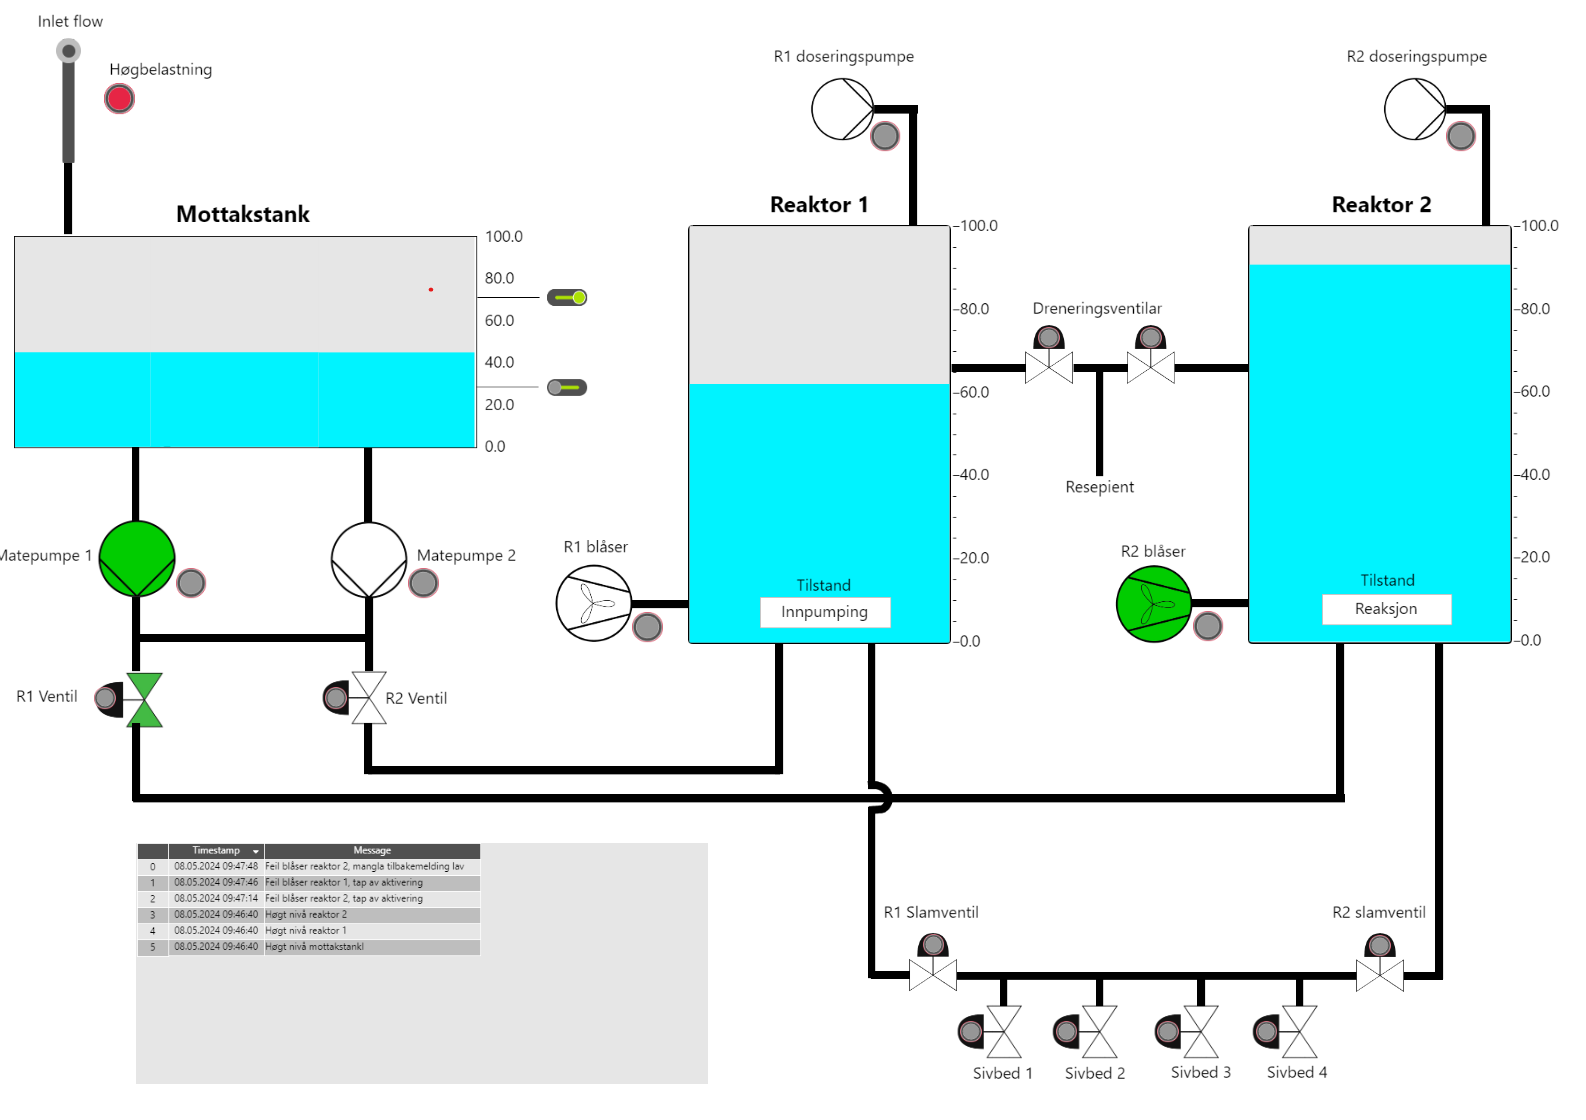
\includegraphics[scale=0.45]{Bilder/Simuleringsbilde.png}
    \caption{Oppsett av simuleringsvindauge}\label{fig:Simulering}
\end{figure}

\newpage

\subsection{Resultat}

Som forventa dukka det opp avvik og ``bugs'' når vi starta med simuleringa.
Nokre av desse var av mindre betydning og blei utbetra undervegs i prosessen, som t.d. den tiltenkte
reaktorforriglinga som ikkje fungerte på overgangen frå pause til innpumpingssekvens. \newline
Andre avvik krevde meir inngåande arbeid og tilbakevending til programmeringa, der problema som oftast låg i skrivefeil, gløymde logiske operasjonar,
\gls{CFC} koplingar som var plassert feil eller konfigurasjonsfeil.

Simuleringa av programmet var svært vellykka og vi fekk samla masse verdifull informasjon frå anlegget i simulert drift. 
Den visuelle representasjonen var oversiktleg, der ein kunne sjå programmet i drift, og det var enkelt å sjå kva programmet gjorde og oppdage feil. 

Vi verifiserte at programmet i hovudsak fungerer som planlagt og vi er no klare til å gjennomføre ei større simulering,
der vi implementerer dei resterande funksjonsblokkene og siktar mot ein fullskala test.





